\documentclass{article}

\usepackage[final]{neurips_2020}
\usepackage[utf8]{inputenc}
\usepackage[T1]{fontenc}
\usepackage{microtype}
\usepackage{graphicx}
\usepackage{booktabs}
\usepackage{amsmath}
\usepackage{url}
\usepackage[hypertexnames=false]{hyperref}
\usepackage{enumitem}
\usepackage{placeins}
\usepackage{float}

\makeatletter
\renewcommand{\@noticestring}{}
\makeatother

\setlist[itemize]{leftmargin=*,nosep}
\setlist[enumerate]{leftmargin=*,nosep}
\makeatletter
\setlength{\@fptop}{0pt}
\setlength{\@fpbot}{0pt plus 1fil}
\makeatother

\title{RouteDoodle GNN v3: Ordered Safety-Aware Route Snapping on a Street Graph}

\author{%
  \textbf{Saj Patel} \\
  \textbf{Prathamesh Swar} \\
  \textbf{Prakhar Pandar} \\
  {\normalfont Final project for Machine Learning with Graphs}
}

\begin{document}

\maketitle

\begin{abstract}
RouteDoodle converts a hand-drawn route shape into a connected walking route on the Houston street graph. The system treats intersections as nodes, walkable street segments as directed edges, and the user drawing as an ordered sequence of geographic points. RouteGAT v3 scores candidate graph edges from doodle geometry, street context, and crime-exposure features. A shortest-path solver then turns those scores into a graph-valid route, so the final output stays on real streets. On 15 validation doodles, GNN v3 matched Dijkstra closely on shape fit, with average Frechet distance of 105 m versus 104 m, while lowering average crime score from 0.0897 to 0.0841.
\end{abstract}

\section{Introduction}

Most route tools ask for a start point and an end point. RouteDoodle uses a different input. The user sketches the shape of a walk, and the system snaps the sketch to a valid route on the Houston street network. This creates a graph learning problem. The input is an ordered drawing, but the output must be a connected path through graph edges.

The project goal is practical: preserve the intent of a drawn route while reducing exposure to higher-risk street segments when a safer nearby path exists. A distance-only shortest-path baseline gives valid graph paths through the same ordered targets, but it ignores learned edge probabilities and crime-exposure penalties. A pure neural path predictor might follow the sketch, but it risks producing disconnected or off-road geometry. RouteDoodle combines both ideas. RouteGAT v3 predicts edge usefulness, and graph routing uses those predictions as edge costs.

The final system has three deliverables. First, the notebook builds a Houston walking graph and attaches safety features from public crime data. Second, it trains a graph attention model on synthetic ordered route examples. Third, it launches a web app where the user draws a route, compares GNN v3 with Dijkstra, reads metrics, and exports route files.

\section{Related Work and Background}

RouteDoodle combines graph routing, graph representation learning, and map matching. Dijkstra's algorithm gives the distance-only routing baseline and the graph-valid solver \citep{dijkstra1959note}. Map matching work studies how noisy or sparse trajectories align to road networks \citep{newson2009hidden}. RouteDoodle differs because the input is an intended sketch, not a measured GPS trace. Graph attention networks learn node representations through learned neighbor weights \citep{velickovic2018graph}. PyTorch Geometric provides graph data objects and model layers \citep{fey2019fast}. OSMnx downloads and stores OpenStreetMap street networks \citep{boeing2017osmnx,openstreetmap}. NetworkX handles traversal and shortest paths \citep{hagberg2008exploring}. Discrete Frechet distance measures route-shape error \citep{eiter1994computing}. The crime-exposure layer uses selected incident categories from the FBI Crime Data Explorer and NIBRS data model \citep{fbi_nibrs}.

The project task differs from standard endpoint routing. A normal shortest-path query has a source node \(s\), a destination node \(t\), and an edge weight such as distance. RouteDoodle starts with an ordered polyline \(D=(d_1,\ldots,d_k)\), where each \(d_i\) is a latitude and longitude point drawn by the user. The model must return a route \(R=(e_1,\ldots,e_m)\) on the walking graph \(G=(V,E)\). The route should stay connected, follow the drawn shape in order, and prefer lower-risk edges when the graph offers an alternative.

The key design decision is to use the learned model as a cost model, not as a direct route generator. A direct generator would need to output an ordered edge list and guarantee that consecutive edges touch. RouteDoodle avoids that fragile step. The GNN scores candidate edges, and shortest-path routing builds the final route. This keeps the output connected and reproducible while letting the model encode shape and safety preferences.

The Dijkstra comparison remains important because it isolates the value of the learned cost. Both methods use the same graph crop and ordered target points. Dijkstra uses distance weights only. GNN v3 changes the edge impedance using learned probabilities, crime score, and amenity proxies. Any difference in output comes from the cost function, not from a different map or route postprocessor.

\section{Data and Graph Construction}

The notebook stores the base walking graph at \texttt{artifacts/houston\_walk\_graph.graphml}. OSMnx downloads the Houston walk network, projects it to a metric coordinate system for distance calculations, and caches it under \texttt{cache/}. Intersections become nodes. Walkable street segments become directed edges with geometry and length. The submitted graph artifact is 293 MB and contains 257,527 nodes and 739,538 directed edges in EPSG:4326 before metric projection.

The graph construction path has four steps. First, the notebook loads the cached GraphML file if it exists and is not a Git LFS pointer. Second, it checks graph usability by reading nodes, edges, geometry, and coordinate reference system fields. Third, it keeps the largest connected walkable component so routing queries do not break on isolated map fragments. Fourth, it saves the cleaned graph back to the artifact path. This check matters because the web app depends on a live route call. A missing geometry field or an empty graph would fail only after the user draws a path.

The crime-exposure graph adds edge-level incident features. The notebook reads \texttt{artifacts/NIBRSPublicView2025.csv}, a 240,696-row Houston incident table spanning 2025-01-01 through 2025-12-31. It filters 20,924 geocoded records from aggravated assault, robbery, and weapon law violations, then maps them to severity weights of 1.0, 0.9, and 0.6. It projects incidents and street geometry to EPSG:32615, computes a severity-weighted incident density within 75 m of each edge, and computes danger overlap with a 10 m buffer around dangerous areas. The cached danger artifact stores 781,524 edges and reports a 95th percentile crime normalization value of 7.1261.

The crime score is edge based. For each street segment, the builder searches incidents within the radius, applies category weights, and normalizes the total by the cached 95th percentile value. A street segment near multiple severe incidents receives a higher score. A segment outside the radius receives zero. Danger overlap measures how much of the edge geometry falls inside the danger buffer. These two values give the model separate signals: nearby incident density and direct overlap with buffered risk areas.

Each graph example uses local node features, edge features, and a global doodle embedding:
\begin{itemize}
  \item Local node features: distance to the doodle, normalized latitude, normalized longitude, and node degree.
  \item Edge features: normalized length, crime score, danger overlap, lighting proxy, sidewalk proxy, and crossing proxy.
  \item Doodle context: a 32-dimensional embedding tiled across nodes inside RouteGAT v3.
\end{itemize}
If the incident files are missing, the notebook keeps the same schema and fills exposure values with zeros. That fallback keeps the route pipeline runnable, but it disables crime-aware scoring.

At app time, the full Houston graph is too large for every route request. The server crops a local subgraph around the doodle. The long example in Figure \ref{fig:app} used 18 input points, simplified them to 15 ordered targets, and routed on a local graph with 6,359 nodes and 20,022 edges. The crop keeps inference interactive while preserving enough street alternatives for the learned exposure cost to matter.

\begin{table}[t]
  \centering
  \caption{Core artifacts for the full cached run. These files let a reader reproduce the final workflow without rebuilding the expensive stages.}
  \label{tab:artifacts}
  \small
  \begin{tabular}{lll}
    \toprule
    Artifact & Role & Observed size \\
    \midrule
    \texttt{houston\_walk\_graph.graphml} & Houston walking graph & 293 MB \\
    \texttt{NIBRSPublicView2025.csv} & public crime source table & 33 MB \\
    \texttt{houston\_danger\_v3.pkl} & safety-annotated graph & 181 MB \\
    \texttt{pyg\_dataset\_v3\_full.pkl} & PyG training examples & 1.3 GB \\
    \texttt{routegat\_v3\_full.pt} & trained RouteGAT v3 checkpoint & 1.8 MB \\
    \bottomrule
  \end{tabular}
\end{table}

\section{Synthetic Route Generation}

The model trains on synthetic route pairs because the project needs many ordered doodle-to-route examples. The full profile uses seed-controlled generation with 1,000 samples. For each sample, the notebook picks 4 to 7 graph waypoints, enforces at least 150 m between waypoints, rejects waypoint gaps above 700 m, and keeps final routes between 1.0 km and 6.0 km with at least 25 route nodes. It then traces the shortest route through those waypoints.

Each synthetic sample follows a fixed process. The sampler chooses a start node, adds waypoints that are far enough apart to create a visible shape but close enough that the graph route stays local, routes between consecutive waypoints, and concatenates those pieces. If any pair is disconnected, too short, too long, or too sparse, the sampler rejects the sample and tries another set of waypoints. The full profile allows up to 500 attempts per sample and saves progress every 25 samples.

The notebook turns each true route into a doodle by resampling the route geometry to 100 points and perturbing it into a sketch-like polyline. The perturbation makes the learning problem closer to the app input. A hand-drawn route does not lie exactly on the street centerline. It cuts corners, drifts across blocks, and contains uneven point spacing. The synthetic doodle keeps the same ordered shape but removes the exact graph-edge alignment.

The dataset stores 16 ordered anchors with a 35 m anchor bandwidth. These anchors divide the doodle into route progress checkpoints. For example, an edge near anchor 3 should explain an early part of the route, while an edge near anchor 13 should explain a later part. This prevents the model from treating the route as an unordered heatmap. The positive edge label marks true-route edges. Negative labels come from nearby graph edges inside the local crop, which gives the model hard alternatives such as parallel streets, adjacent blocks, and shortcuts that look plausible but do not match the route.

The final PyG object contains node features, edge indices, edge attributes, edge labels, doodle features, anchor targets, and metadata for route reconstruction. The cached full dataset is \texttt{artifacts/pyg\_dataset\_v3\_full.pkl}. The reported validation metrics use 15 synthetic doodles from the full profile, so they test the v3 data path rather than the smoke configuration.

\section{RouteDoodle GNN v3 Method}

Figure \ref{fig:pipeline} summarizes the model path. The app or notebook starts with an ordered doodle. The route builder crops a graph around the doodle, computes node and edge features, and sends the example through RouteGAT v3. A one-dimensional convolutional doodle encoder summarizes the ordered polyline. Graph attention layers combine that doodle embedding with local node features. The final edge scorer then combines source-node state, destination-node state, and edge features to predict a probability for each candidate edge.

\begin{figure}[t]
  \centering
  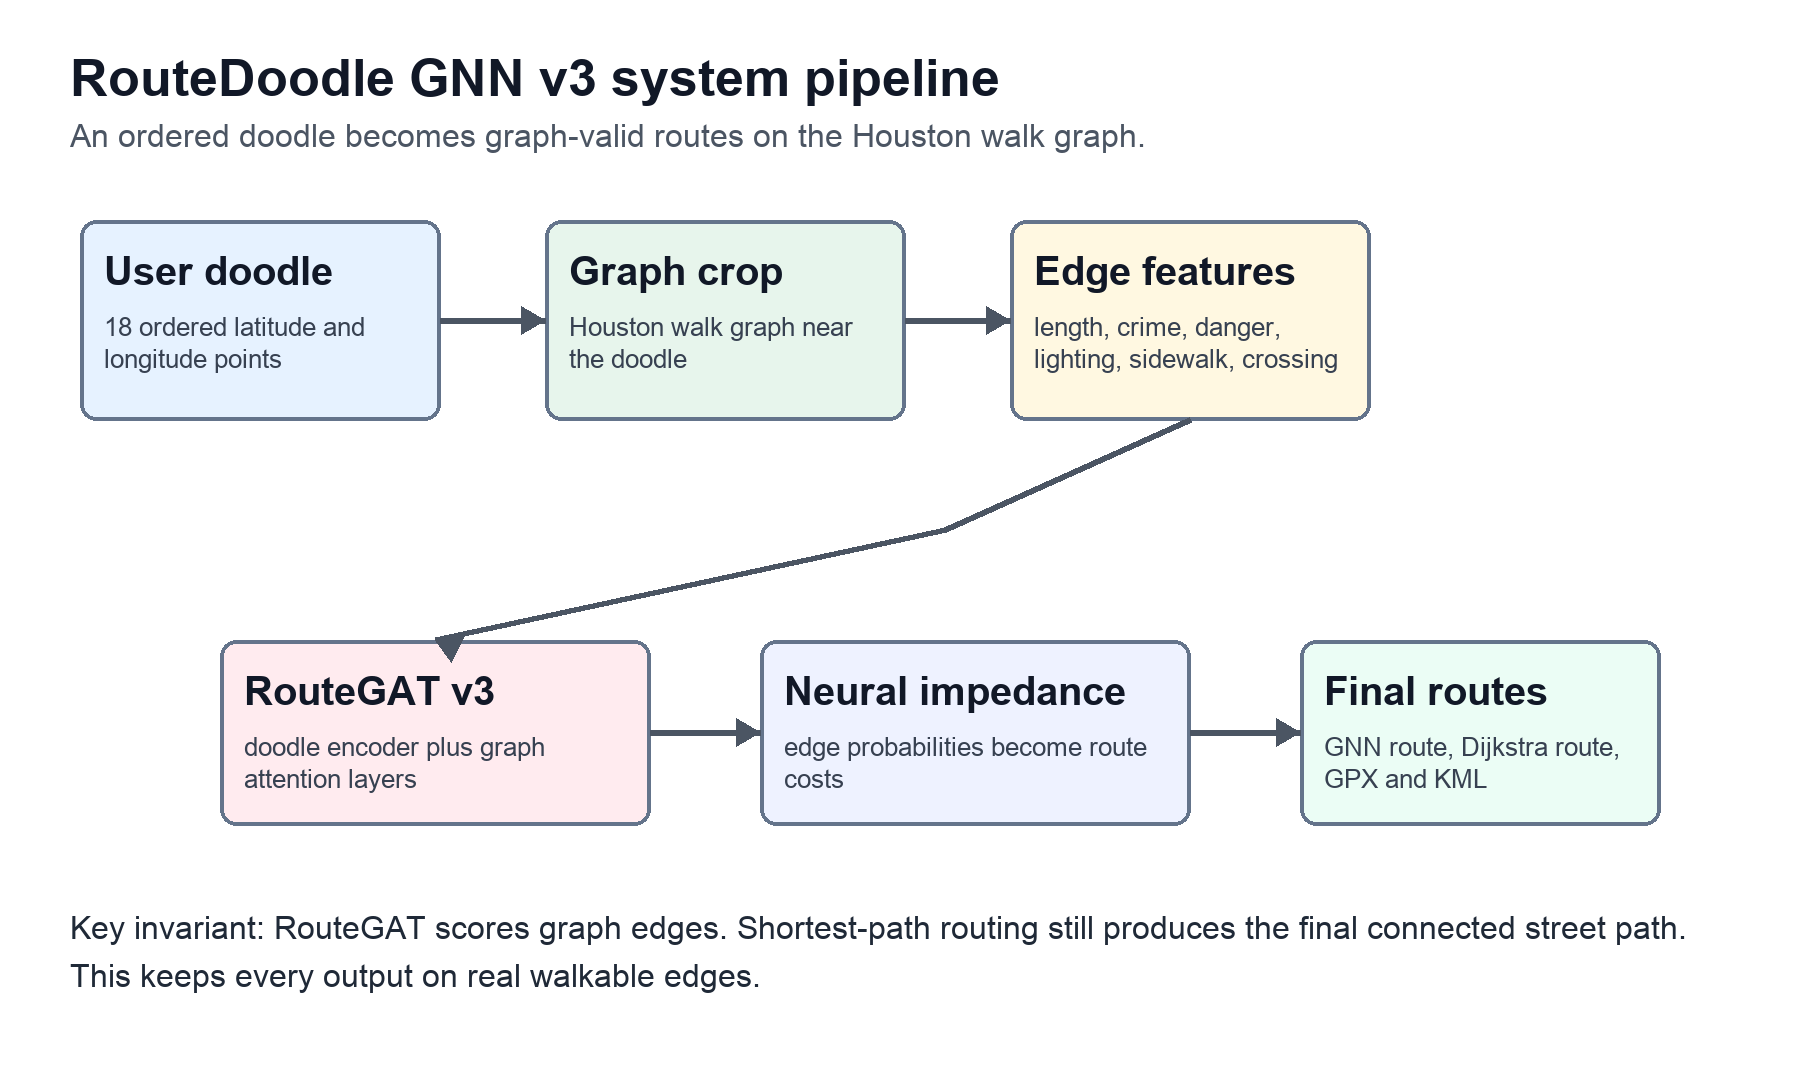
\includegraphics[width=\linewidth]{figures/pipeline.png}
  \caption{RouteDoodle scores graph edges from an ordered doodle, then uses graph routing to produce connected street routes.}
  \label{fig:pipeline}
\end{figure}

The doodle encoder receives the ordered route sketch as a sequence rather than an image. It processes resampled coordinate and distance channels with one-dimensional convolutions, then pools the sequence into a fixed-length embedding. This representation preserves order while staying small enough to concatenate into every graph example. The graph branch uses node features for local position and topology. Edge features enter the scorer so length and safety affect edge probability directly.

The full model has 155,393 trainable parameters. It uses 6 edge features, three graph attention layers, two 4-head layers, one 2-head output layer, and dropout 0.2. The attention layers let each node read from nearby intersections after the doodle context is concatenated to local node features. The edge scorer receives the source node embedding, destination node embedding, and edge feature vector. This matters because a street segment depends on both endpoints and the segment attributes.

Training uses a multi-term objective:
\begin{equation}
  \mathcal{L} =
  \mathcal{L}_{\mathrm{BCE}} +
  0.2\mathcal{L}_{\mathrm{anchor}} +
  0.4\mathcal{L}_{\mathrm{safety}}.
\end{equation}
The binary cross-entropy term teaches route membership with positive-edge weight 15. The anchor term is mean squared error against the ordered anchor heatmap. The safety term is the mean of predicted edge probability times crime score, so it discourages probability mass on high-crime edges. Training uses seed 42, an 80/20 train-validation split, Adam with learning rate \(10^{-3}\), weight decay \(10^{-4}\), batch size 16, and 15 full-profile epochs. The final run restored \texttt{routegat\_v3\_full.pt}.

At inference time, RouteGAT v3 does not return a path directly. It returns edge probabilities \(P(e)\). The route solver converts those probabilities into a neural impedance weight:
\begin{equation}
  W(e)=
  \mathrm{length}_e
  \frac{1}{P(e)+0.01}
  \frac{1 + 2.5\,\mathrm{crime}_e}{\max(0.75, 1 + 0.25\,\mathrm{amenity}_e)}.
\end{equation}
High model confidence lowers route cost. Crime raises route cost. Amenity proxies lower route cost within a capped range. The solver routes through ordered targets using these weights. This step preserves graph validity because every segment still comes from the walking graph.

The impedance formula gives a concrete behavior. If two nearby streets both follow the doodle, the edge with higher \(P(e)\) receives lower cost. If those two streets have similar probability but one has higher crime score, the safer edge receives lower cost. If a route edge has weak model probability, the inverse probability term makes it expensive even when it is short. The final route therefore balances three pressures: stay near the drawn path, avoid unnecessary distance, and reduce crime exposure when a connected alternative exists.

After routing, the app computes route metrics from the returned geometry. Coverage reports how many ordered targets the route satisfies. Shape error measures distance between route geometry and doodle geometry. Crime and danger aggregate edge safety values along the route. Exposed fraction counts the share of route segments with nonzero exposure. These metrics let the reader compare the learned route and Dijkstra on the same input instead of judging the map image alone.

\section{Working Web Application}

The final notebook launches the app from section \texttt{8.3 Launch full-page web map}. The local URL is \texttt{http://127.0.0.1:8765/}. The captured run reported profile \texttt{full} and artifact version \texttt{v3\_ordered\_safety}. The notebook also exposes a public Cloudflare URL when the runtime permits tunnels.

Figure \ref{fig:app} uses the live local app. The fixed test doodle has 18 input points and simplifies to 15 ordered routing targets. The route spans downtown and central Houston at street scale. The left panel shows route metrics, and the right panel shows the street graph view.

\begin{figure}[t]
  \centering
  \makebox[\linewidth][c]{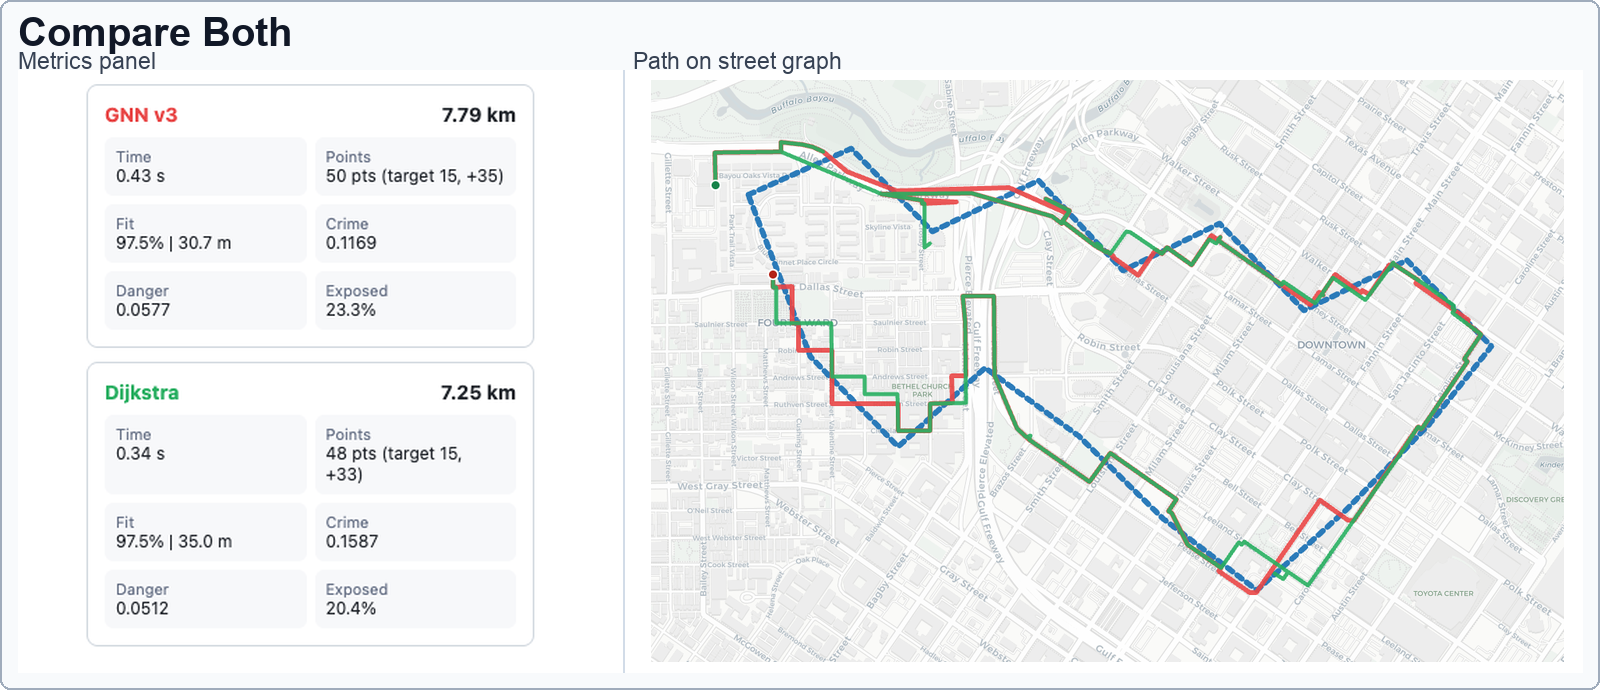
\includegraphics[width=1.12\linewidth,height=0.41\textheight,keepaspectratio]{figures/app_both_row_long.png}}
  \caption{Live app comparison for the long-path example. The blue dashed line is the user doodle, red is GNN v3, and green is Dijkstra.}
  \label{fig:app}
\end{figure}

For this example, the app selected a local subgraph with 6,359 nodes and 20,022 edges. GNN v3 returned a 7.79 km route, or 4.84 miles, with 50 route points, 97.5\% fit, 30.7 m shape error, 0.1169 crime score, 0.0577 danger score, and 23.3\% exposed fraction. Dijkstra returned a 7.25 km route, or 4.51 miles, with 48 route points, 97.5\% fit, 35.0 m shape error, 0.1587 crime score, 0.0512 danger score, and 20.4\% exposed fraction. This example shows how the learned cost changes the chosen streets while keeping the route connected and close to the drawn shape.

Both methods reached 97.5\% fit on this long route, so both preserved the drawn shape. GNN v3 had lower shape error, 30.7 m instead of 35.0 m, and lower average crime score, 0.1169 instead of 0.1587. Dijkstra was shorter by 0.54 km and had slightly lower danger and exposed fraction. The example shows the project behavior: the learned cost produced a valid route close to the sketch and reduced the main crime score, while accepting a longer route and mixed secondary safety metrics.

\FloatBarrier

\section{Experiments and Results}
\label{sec:results}

The final evaluation uses the first 15 validation doodles from the full profile. The dataset split is 800 training examples and 200 validation examples under seed 42. Each sample compares GNN v3 with Dijkstra on the same doodle and local graph. The main shape metric is discrete Frechet distance in meters. The crime-exposure metric is average crime score along the returned route, measured on the route geometry after graph snapping.

\begin{table}[H]
  \centering
  \caption{Validation evaluation on 15 synthetic doodles. Lower Frechet distance and lower crime score are better.}
  \label{tab:results}
  \small
  \begin{tabular}{lcc}
    \toprule
    Metric & GNN v3 & Dijkstra \\
    \midrule
    Average Frechet distance & 105 m & 104 m \\
    Average crime score & 0.0841 & 0.0897 \\
    Shape wins & 1 of 15 & 14 of 15 \\
    Crime wins & 12 of 15 & 0 of 15 \\
    Crime ties & 3 of 15 & 3 of 15 \\
    Output validity & graph path & graph path \\
    \bottomrule
  \end{tabular}
\end{table}

The result supports a specific claim. GNN v3 is not a better pure shape matcher than Dijkstra on this small validation set. The average Frechet distances differ by 1 m, and Dijkstra wins most shape comparisons under the strict printed comparison. The learned route cost still moves the crime-exposure proxy in the intended direction. Average crime score drops by 0.0056, or about 6.2\%, while every output remains a graph-valid route.

This result should be interpreted as validation evidence for a safety-aware route snapping system, not as proof that graph learning alone caused the crime-score drop. The GNN impedance mixes learned probabilities, a hand-coded crime multiplier, and amenity proxies. A stronger study would add a true test split, real user sketches, repeated seeds, and ablations such as distance-only Dijkstra, crime-aware Dijkstra without \(P(e)\), and \(P(e)\)-only GNN routing.

\section{Challenges and Discussion}

The first challenge was graph validity. A doodle is continuous, but a legal route must follow connected graph edges. The neural-impedance design addresses this by using RouteGAT v3 for edge scoring and shortest-path routing for final path construction. The second challenge was order. A route is a sequence, not a bag of edges. The v3 dataset stores ordered anchors, and the loss includes an anchor term so the model learns where each part of the doodle belongs along the path.

The third challenge was crime-exposure feature quality. Crime incidents are spatial, sparse, and category-dependent. The current score is useful for comparison inside this project, but it is not a personal safety guarantee. It does not model lighting conditions in real time, reporting bias, time of day, or pedestrian traffic. The fourth challenge was artifact size. The full local artifact set is about 2.9 GB, and the PyG dataset is the largest file. The notebook handles this through a local-cache-first workflow that rejects Git LFS pointer files, tries Git LFS assets, and rebuilds missing components when needed.

\section{Reproducibility and Conclusion}

The public implementation is available at \url{https://github.com/sajpatel15/comp_559} at report commit \texttt{63f5b05}. The project has one required entry point, \texttt{routedoodle\_gnn\_v2.ipynb}. A full cached run uses \texttt{ROUTEDOODLE\_RUN\_PROFILE=full}, restores \texttt{houston\_walk\_graph.graphml}, \texttt{houston\_danger\_v3.pkl}, \texttt{pyg\_dataset\_v3\_full.pkl}, and \texttt{routegat\_v3\_full.pt}, launches the app on port 8765, and writes GPX and KML outputs under \texttt{outputs/}. The README gives the full Colab, Jupyter, public URL, cache, Git LFS, and rebuild instructions.

RouteDoodle shows that an ordered sketch can be converted into a connected street-graph route while using graph learning to reshape route costs. The strongest evidence is graph validity, close shape fit, and lower validation crime score. The main limitation is attribution: future work should separate learned probability effects from hand-coded exposure penalties and evaluate on larger real-doodle test sets.

\FloatBarrier

\section{Equal Contributions}

The team split ownership evenly across idea formation, prototype work, research, implementation, evaluation, and report delivery. Saj Patel led final system integration, refined the prototype into the final notebook, hardened the app workflow, and completed the final reproduction path. Prathamesh Swar proposed the initial RouteDoodle idea, built the early prototype direction, and helped define the graph route-snapping problem. Prakhar Pandar supported research, idea iteration, code development, evaluation, and system improvement. Together, the three members share ownership of the final concept, model, app, evaluation, and report.

\section*{Acknowledgments}

The implementation uses OpenStreetMap data through OSMnx, public incident categories from the FBI Crime Data Explorer, PyTorch Geometric for graph learning, and NetworkX for graph routing.

\bibliographystyle{plainnat}
\bibliography{references}

\end{document}
